\documentclass[journal,12pt,twocolumn]{IEEEtran}

\usepackage{setspace}
\usepackage{gensymb}
\singlespacing
\usepackage[cmex10]{amsmath}

\usepackage{amsthm}

\usepackage{mathrsfs}
\usepackage{txfonts}
\usepackage{stfloats}
\usepackage{bm}
\usepackage{cite}
\usepackage{cases}
\usepackage{subfig}

\usepackage{longtable}
\usepackage{multirow}

\usepackage{enumitem}
\usepackage{mathtools}
\usepackage{steinmetz}
\usepackage{tikz}
\usepackage{circuitikz}
\usepackage{verbatim}
\usepackage{tfrupee}
\usepackage[breaklinks=true]{hyperref}
\usepackage{graphicx}
\usepackage{tkz-euclide}

\usetikzlibrary{calc,math}
\usepackage{listings}
    \usepackage{color}                                            %%
    \usepackage{array}                                            %%
    \usepackage{longtable}                                        %%
    \usepackage{calc}                                             %%
    \usepackage{multirow}                                         %%
    \usepackage{hhline}                                           %%
    \usepackage{ifthen}                                           %%
    \usepackage{lscape}     
\usepackage{multicol}
\usepackage{chngcntr}
\usepackage{float}
\restylefloat{table}

\DeclareMathOperator*{\Res}{Res}

\renewcommand\thesection{\arabic{section}}
\renewcommand\thesubsection{\thesection.\arabic{subsection}}
\renewcommand\thesubsubsection{\thesubsection.\arabic{subsubsection}}

\renewcommand\thesectiondis{\arabic{section}}
\renewcommand\thesubsectiondis{\thesectiondis.\arabic{subsection}}
\renewcommand\thesubsubsectiondis{\thesubsectiondis.\arabic{subsubsection}}


\hyphenation{op-tical net-works semi-conduc-tor}
\def\inputGnumericTable{}                                 %%

\lstset{
%language=C,
frame=single, 
breaklines=true,
columns=fullflexible
}
\begin{document}

\newcommand{\BEQA}{\begin{eqnarray}}
\newcommand{\EEQA}{\end{eqnarray}}
\newcommand{\define}{\stackrel{\triangle}{=}}
\bibliographystyle{IEEEtran}
\raggedbottom
\setlength{\parindent}{0pt}
\providecommand{\mbf}{\mathbf}
\providecommand{\pr}[1]{\ensuremath{\Pr\left(#1\right)}}
\providecommand{\qfunc}[1]{\ensuremath{Q\left(#1\right)}}
\providecommand{\sbrak}[1]{\ensuremath{{}\left[#1\right]}}
\providecommand{\lsbrak}[1]{\ensuremath{{}\left[#1\right.}}
\providecommand{\rsbrak}[1]{\ensuremath{{}\left.#1\right]}}
\providecommand{\brak}[1]{\ensuremath{\left(#1\right)}}
\providecommand{\lbrak}[1]{\ensuremath{\left(#1\right.}}
\providecommand{\rbrak}[1]{\ensuremath{\left.#1\right)}}
\providecommand{\cbrak}[1]{\ensuremath{\left\{#1\right\}}}
\providecommand{\lcbrak}[1]{\ensuremath{\left\{#1\right.}}
\providecommand{\rcbrak}[1]{\ensuremath{\left.#1\right\}}}
\theoremstyle{remark}
\newtheorem{rem}{Remark}
\newcommand{\sgn}{\mathop{\mathrm{sgn}}}
\newcommand*{\permcomb}[4][0mu]{{{}^{#3}\mkern#1#2_{#4}}}
\newcommand*{\perm}[1][-3mu]{\permcomb[#1]{P}}
\newcommand*{\comb}[1][-1mu]{\permcomb[#1]{C}}
\providecommand{\abs}[1]{\vert#1\vert}
\providecommand{\res}[1]{\Res\displaylimits_{#1}} 
\providecommand{\norm}[1]{\lVert#1\rVert}
%\providecommand{\norm}[1]{\lVert#1\rVert}
\providecommand{\mtx}[1]{\mathbf{#1}}
\providecommand{\mean}[1]{E[ #1 ]}
\providecommand{\fourier}{\overset{\mathcal{F}}{ \rightleftharpoons}}
%\providecommand{\hilbert}{\overset{\mathcal{H}}{ \rightleftharpoons}}
\providecommand{\system}{\overset{\mathcal{H}}{ \longleftrightarrow}}
	%\newcommand{\solution}[2]{\textbf{Solution:}{#1}}
\newcommand{\solution}{\noindent \textbf{Solution: }}
\newcommand{\cosec}{\,\text{cosec}\,}
\providecommand{\dec}[2]{\ensuremath{\overset{#1}{\underset{#2}{\gtrless}}}}
\newcommand{\myvec}[1]{\ensuremath{\begin{pmatrix}#1\end{pmatrix}}}
\newcommand{\mydet}[1]{\ensuremath{\begin{vmatrix}#1\end{vmatrix}}}
\numberwithin{equation}{subsection}
\makeatletter
\@addtoreset{figure}{problem}
\makeatother
\let\StandardTheFigure\thefigure
\let\vec\mathbf
\renewcommand{\thefigure}{\theproblem}
\def\putbox#1#2#3{\makebox[0in][l]{\makebox[#1][l]{}\raisebox{\baselineskip}[0in][0in]{\raisebox{#2}[0in][0in]{#3}}}}
     \def\rightbox#1{\makebox[0in][r]{#1}}
     \def\centbox#1{\makebox[0in]{#1}}
     \def\topbox#1{\raisebox{-\baselineskip}[0in][0in]{#1}}
     \def\midbox#1{\raisebox{-0.5\baselineskip}[0in][0in]{#1}}
\vspace{3cm}
\title{AI1103 ASSIGNMENT 4}
\author{Name:MANNAM SARANDEEP,Rollno:CS20BTECH11030}
\maketitle
\newpage
\bigskip
\renewcommand{\thefigure}{\theenumi}
\renewcommand{\thetable}{\theenumi}

Download the python code from 
\begin{lstlisting}
https://github.com/sarandeepmannam/ASSIGNMENT4/blob/main/Assignment4.py
\end{lstlisting}
%
and latex-tikz code from 
%
\begin{lstlisting}
https://github.com/sarandeepmannam/ASSIGNMENT4/blob/main/Assignment4.tex
\end{lstlisting}
\section{Question-CSIR UGC NET June 2012,Q.50}
Let $X_{1},X_{2},....$ be i.i.d N(1,1) random variables.Let $S_{n}=X_{1}^{2}+X_{2}^2+...+X_{n}^{2}$ for $n\ge1$.Then $$\lim_{n \to \infty}{\frac{Var\brak{S_{n}}}{n}}=$$
\begin{enumerate}[label = (\Alph*)]
\item  $4$
\item  $6$
\item  $1$
\item  $0$
\end{enumerate}

\section{Solution-CSIR UGC NET June 2012,Q.50}

If two random variables $X,Y$ are independent then $X^2,Y^2$ are also independent.
Since $X_{1},X_{2},X_{3},...$ are mutually independent random variables therefore the random variables $X_{1}^{2},X_{2}^{2},X_{3}^{2},....$  are also mutually independent.

\begin{align}
    S_{n}=X_{1}^2+X_{2}^2+X_{3}^2+......X_{n}^2
\end{align}
We know that if X and Y are independent random variables $Var(X+Y)=Var(X)+Var(Y)$.
\\Therefore,
\begin{align}
    Var\brak{S_{n}}=Var\brak{X_{1}^2}+Var\brak{X_{2}^2}+..Var\brak{X_{n}^2}
\end{align}
Since $X_{1},X_{2},..X_{n}$ are identically distributed random variables therefore the random variables $X_{1}^2,X_{2}^2,...X_{n}^2$ are also identical.So,
\begin{align}
    Var\brak{X_{1}^2}=Var\brak{X_{2}^2}=...=Var\brak{X_{n}^2}
\end{align}
Now we find the variance of $X_{1}^2$.
\begin{align}
    Var(X_{1}^2)=E(X_{1}^4)-(E(X_{1}^2))^2
\end{align}
But we don't know the values of $E(x_{1}^2)$ and $E(X_{1}^4)$
First we find the value of $E(x_{1}^2)$. 
\begin{align}
    Var(X_{1})=E(X_{1}^2)-(E(X_{1}))^2
\end{align}
Since $X_{1}$ is a N(1,1) random variable $E(X_{1})=1$ and $Var(X_{1})=1$.Therefore,
\begin{align}
    E(X_{1}^2)-(1)^2&=1
 \\  E(X_{1}^2)&=2
\end{align}
Now we find the value of $E(X_{1}^4)$.
\\Since $X_{1}$ is a $N(1,1)$ random variable pdf of $X_{1}$ will be 
\begin{align}
    f(X_{1})=\frac{1}{\sqrt{2\pi}}\brak{e^{-\frac{(X_{1}-1)^2}{2}}}
\end{align}
\begin{figure}[h]
    \centering
    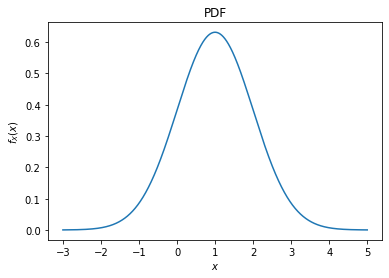
\includegraphics[width=\columnwidth]{PDF.png}
    \caption{PDF of $X_{1},X_{2},..$}
    \label{fig:my_label}
\end{figure}

Now expected value of $X_{1}^{4}$ will be,
\begin{align}
   E(X_{1}^4)&=\int\limits_{-\infty}^{+\infty}X_{1}^{4}f(X_{1})\,dX_{1}
\\   &=\int\limits_{-\infty}^{+\infty}X_{1}^{4}\brak{\frac{1}{\sqrt{2\pi}}\brak{e^{-\frac{(X_{1}-1)^2}{2}}}}\,dX_{1}
\end{align}
Now put $X_{1}-1=t$,
\begin{align}
    E(X_{1}^4)&=\frac{1}{\sqrt{2\pi}}\int\limits_{-\infty}^{+\infty}(t+1)^{4}\brak{e^{-\frac{t^{2}}{2}}}\,dt
\\ &=\frac{1}{\sqrt{2\pi}}\int\limits_{-\infty}^{+\infty}(t^{4}+4t^{3}+6t^{2}+4t+1)\brak{e^{-\frac{t^{2}}{2}}}\,dt
\end{align}
Since $\int\limits_{-\infty}^{+\infty}4t^3\brak{e^{-\frac{t^{2}}{2}}}\,dt$ and $\int\limits_{-\infty}^{+\infty}4t\brak{e^{-\frac{t^{2}}{2}}}\,dt$ are equal to zero,the equation will get reduced to
\begin{align}
    E(X_{1}^4)&=\frac{1}{\sqrt{2\pi}}\int\limits_{-\infty}^{+\infty}(t^{4}+6t^{2}+1)\brak{e^{-\frac{t^{2}}{2}}}\,dt
\end{align}
Now put $\frac{t}{\sqrt{2}}=x$,
\begin{align}
    E(X_{1}^4)&=\frac{1}{\sqrt{\pi}}\int\limits_{-\infty}^{+\infty}(4x^{4}+12x^{2}+1)\brak{e^{-x^{2}}}\,dx
\end{align}
We know that,
\begin{align}
\int\limits_{-\infty}^{+\infty}\brak{e^{-ax^{2}}}\,dx&=\frac{\sqrt{\pi}}{\sqrt{a}}
\\\frac{d\brak{\int\limits_{-\infty}^{+\infty}\brak{e^{-ax^{2}}}\,dx}}{da}&=\frac{d}{da}\brak{\frac{\sqrt{\pi}}{\sqrt{a}}}
\\\int\limits_{-\infty}^{+\infty}x^{2}\brak{e^{-ax^{2}}}\,dx&=\frac{\sqrt{\pi}}{2\sqrt{a^3}}
\end{align}
similarly,
\begin{align}
    \int\limits_{-\infty}^{+\infty}x^{4}\brak{e^{-ax^{2}}}\,dx&=\frac{3\sqrt{\pi}}{4\sqrt{a^5}}
\end{align}
Using (2.0.15),(2.0.17) and (2.0.18) in (2.0.14) we get,
\begin{align}
     E(X_{1}^4)&=\frac{1}{\sqrt{\pi}}\brak{4\brak{\frac{3\sqrt{\pi}}{4}}+12\brak{\frac{\sqrt{\pi}}{2}}+\sqrt{\pi}}
     \\&=3+6+1
    \\\implies  E(X_{1}^4)&=10
\end{align}
Substituting (2.0.21),(2.0.7) in (2.0.4) we get,
\begin{align}
    Var(X_{1}^{2})&=10-4
    \\\implies Var(X_{1}^{2})&=6
\end{align}
By the equations (2.0.23),(2.0.3) and (2.0.2), we can conclude that 
\begin{align}
    Var(S_{n})=6n
\end{align}
$$\lim_{n \to \infty}{\frac{Var\brak{S_{n}}}{n}}=\lim_{n \to \infty}{\frac{6n}{n}}=\lim_{n \to \infty}{6}=6$$
Hence, option (B) is correct.











\end{document}
